\documentclass[a4paper, 12pt]{article}
\usepackage[total={17cm,25cm}, top=2.5cm, left=2.5cm, right=2.5cm,  includefoot]{geometry}
\usepackage[utf8]{inputenc}
\usepackage{array}
\usepackage{multirow}
\usepackage{hhline}
\usepackage{gensymb}
\usepackage{graphicx}
\graphicspath{ {} }
\usepackage[czech]{babel}
\usepackage{enumitem}
\usepackage{pdfpages}
\usepackage{amsmath}
\usepackage{verbatim}
\usepackage{listings}
\usepackage{hyperref}
\usepackage{amssymb}


\pagestyle{empty} % vypne číslování stránek




%\usepackage[OT2,OT1]{fontenc}
\newcommand\cyr
{
\renewcommand\rmdefault{wncyr}
\renewcommand\sfdefault{wncyss}
\renewcommand\encodingdefault{OT2}
\normalfont
\selectfont
}
\DeclareTextFontCommand{\textcyr}{\cyr}
\def\cprime{\char"7E }
\def\cdprime{\char"7F }
\def\eoborotnoye{\char’013}
\def\Eoborotnoye{\char’003}


\begin{document}



\begin{titlepage}
\begin{center}
\noindent
\Large \textbf{České vysoké učení technické v Praze }\\ Fakulta stavební
\vspace{5cm}

\huge

%vložení loga cvut
%\begin{figure}[h!]
%	\centering
%	\includegraphics[width=7cm]{logo.png}
%\end{figure}

\vspace{0.5cm}

155ADKG: Množinové operace s polygony \\

\vspace{10cm}




\Large
Michael Kala\\
Anna Zemánková \\

\end{center}

\end{titlepage}




\pagestyle{plain}     % zapne obyčejné číslování
\setcounter{page}{1}  % nastaví čítač stránek znovu od jedné

%\tableofcontents
%\newpage

\section{Zadání}

\begin{figure}[h!]
	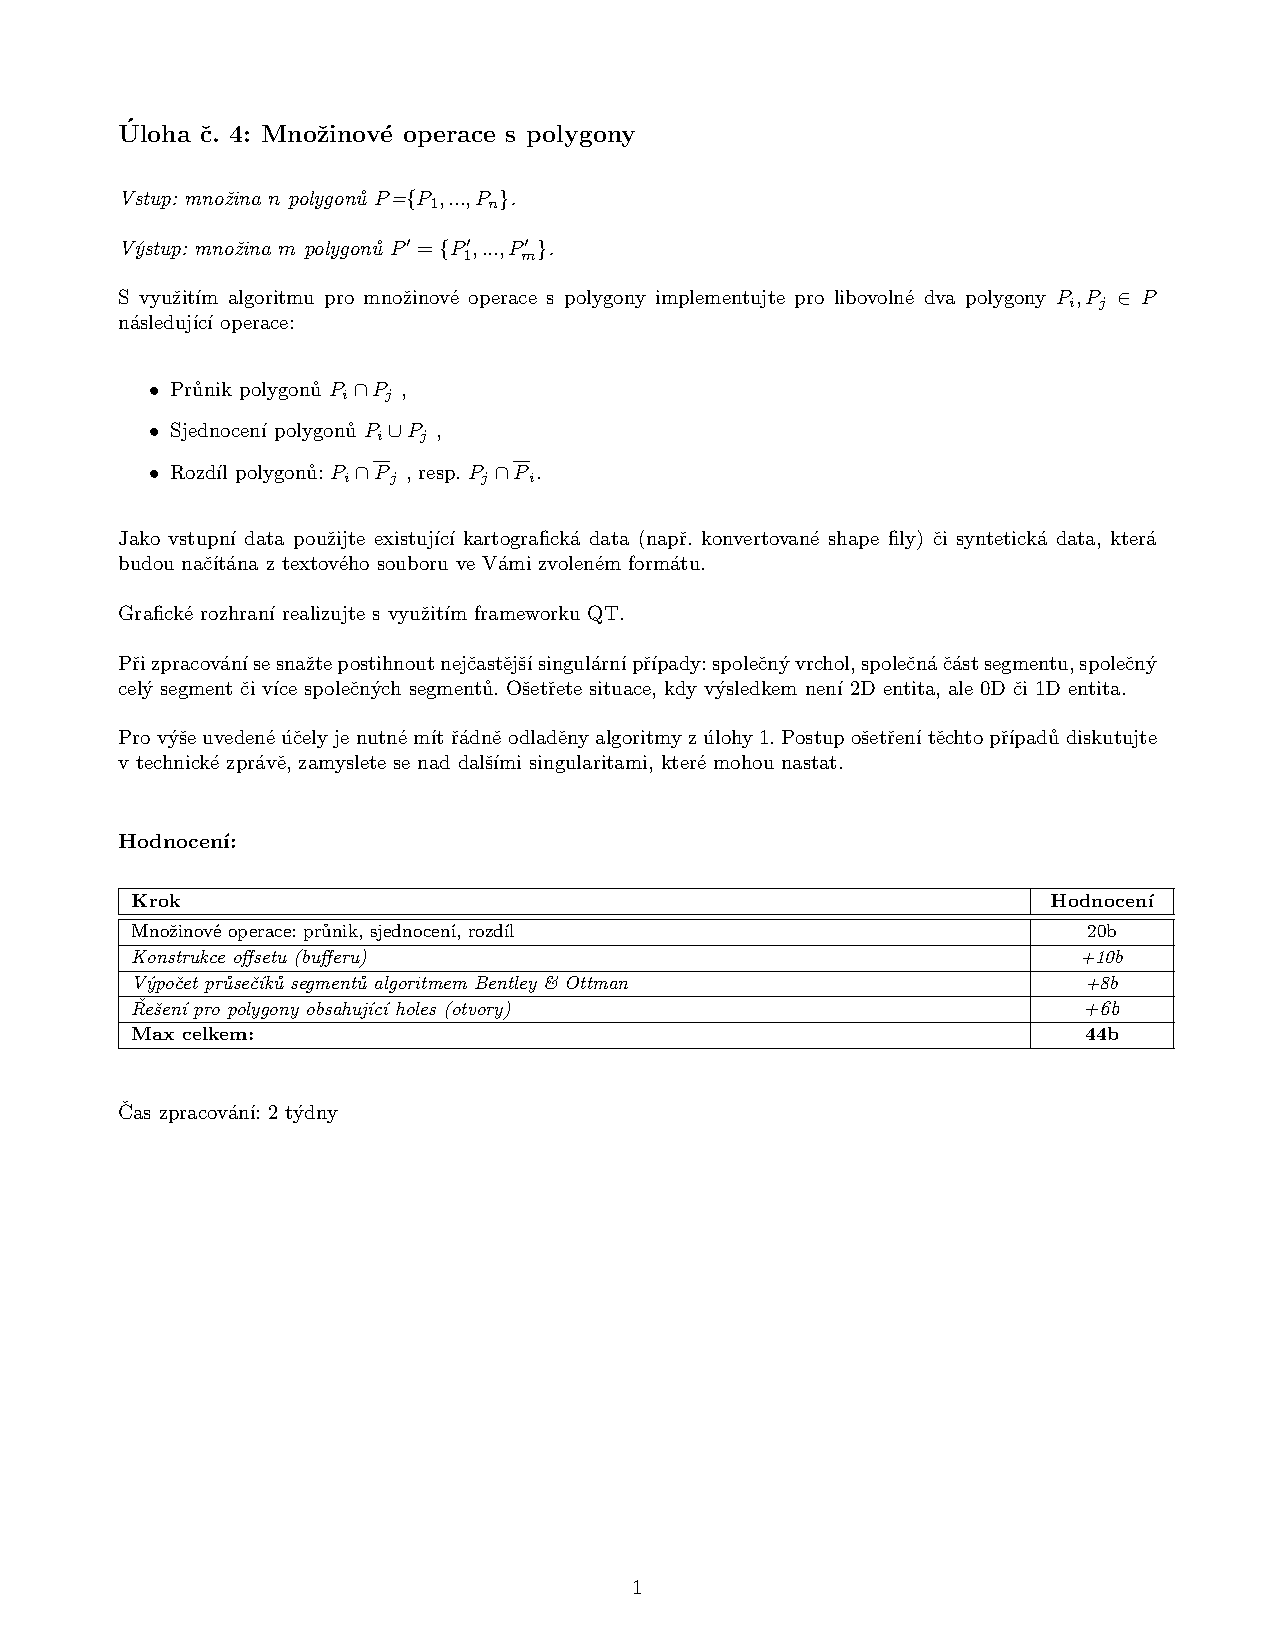
\includegraphics[clip, trim=0cm 4cm 0cm 3cm, width=1.0\textwidth]{zadani.pdf}
\end{figure}


\section{Údaje o bonusových úlohách}

V rámci této úlohy nebyly zpracovány žádné bonusy.



\clearpage

\section{Popis a rozbor problému}
Mějme dva polygony A $\{p_i\}$ a B $\{p_j\}$.\\

Množinové operace:
\begin{itemize}
\item Sjednocení (Union): $C = A \cup B$
\item Průnik (Intersection): $C = A \cap B$
\item Rozdíl (Difference): $C = A \cap \bar{B}$ nebo $C = B \cap \bar{A}$
\end{itemize}

%OBRÁZEK
\begin{figure}[h]
	\centering
	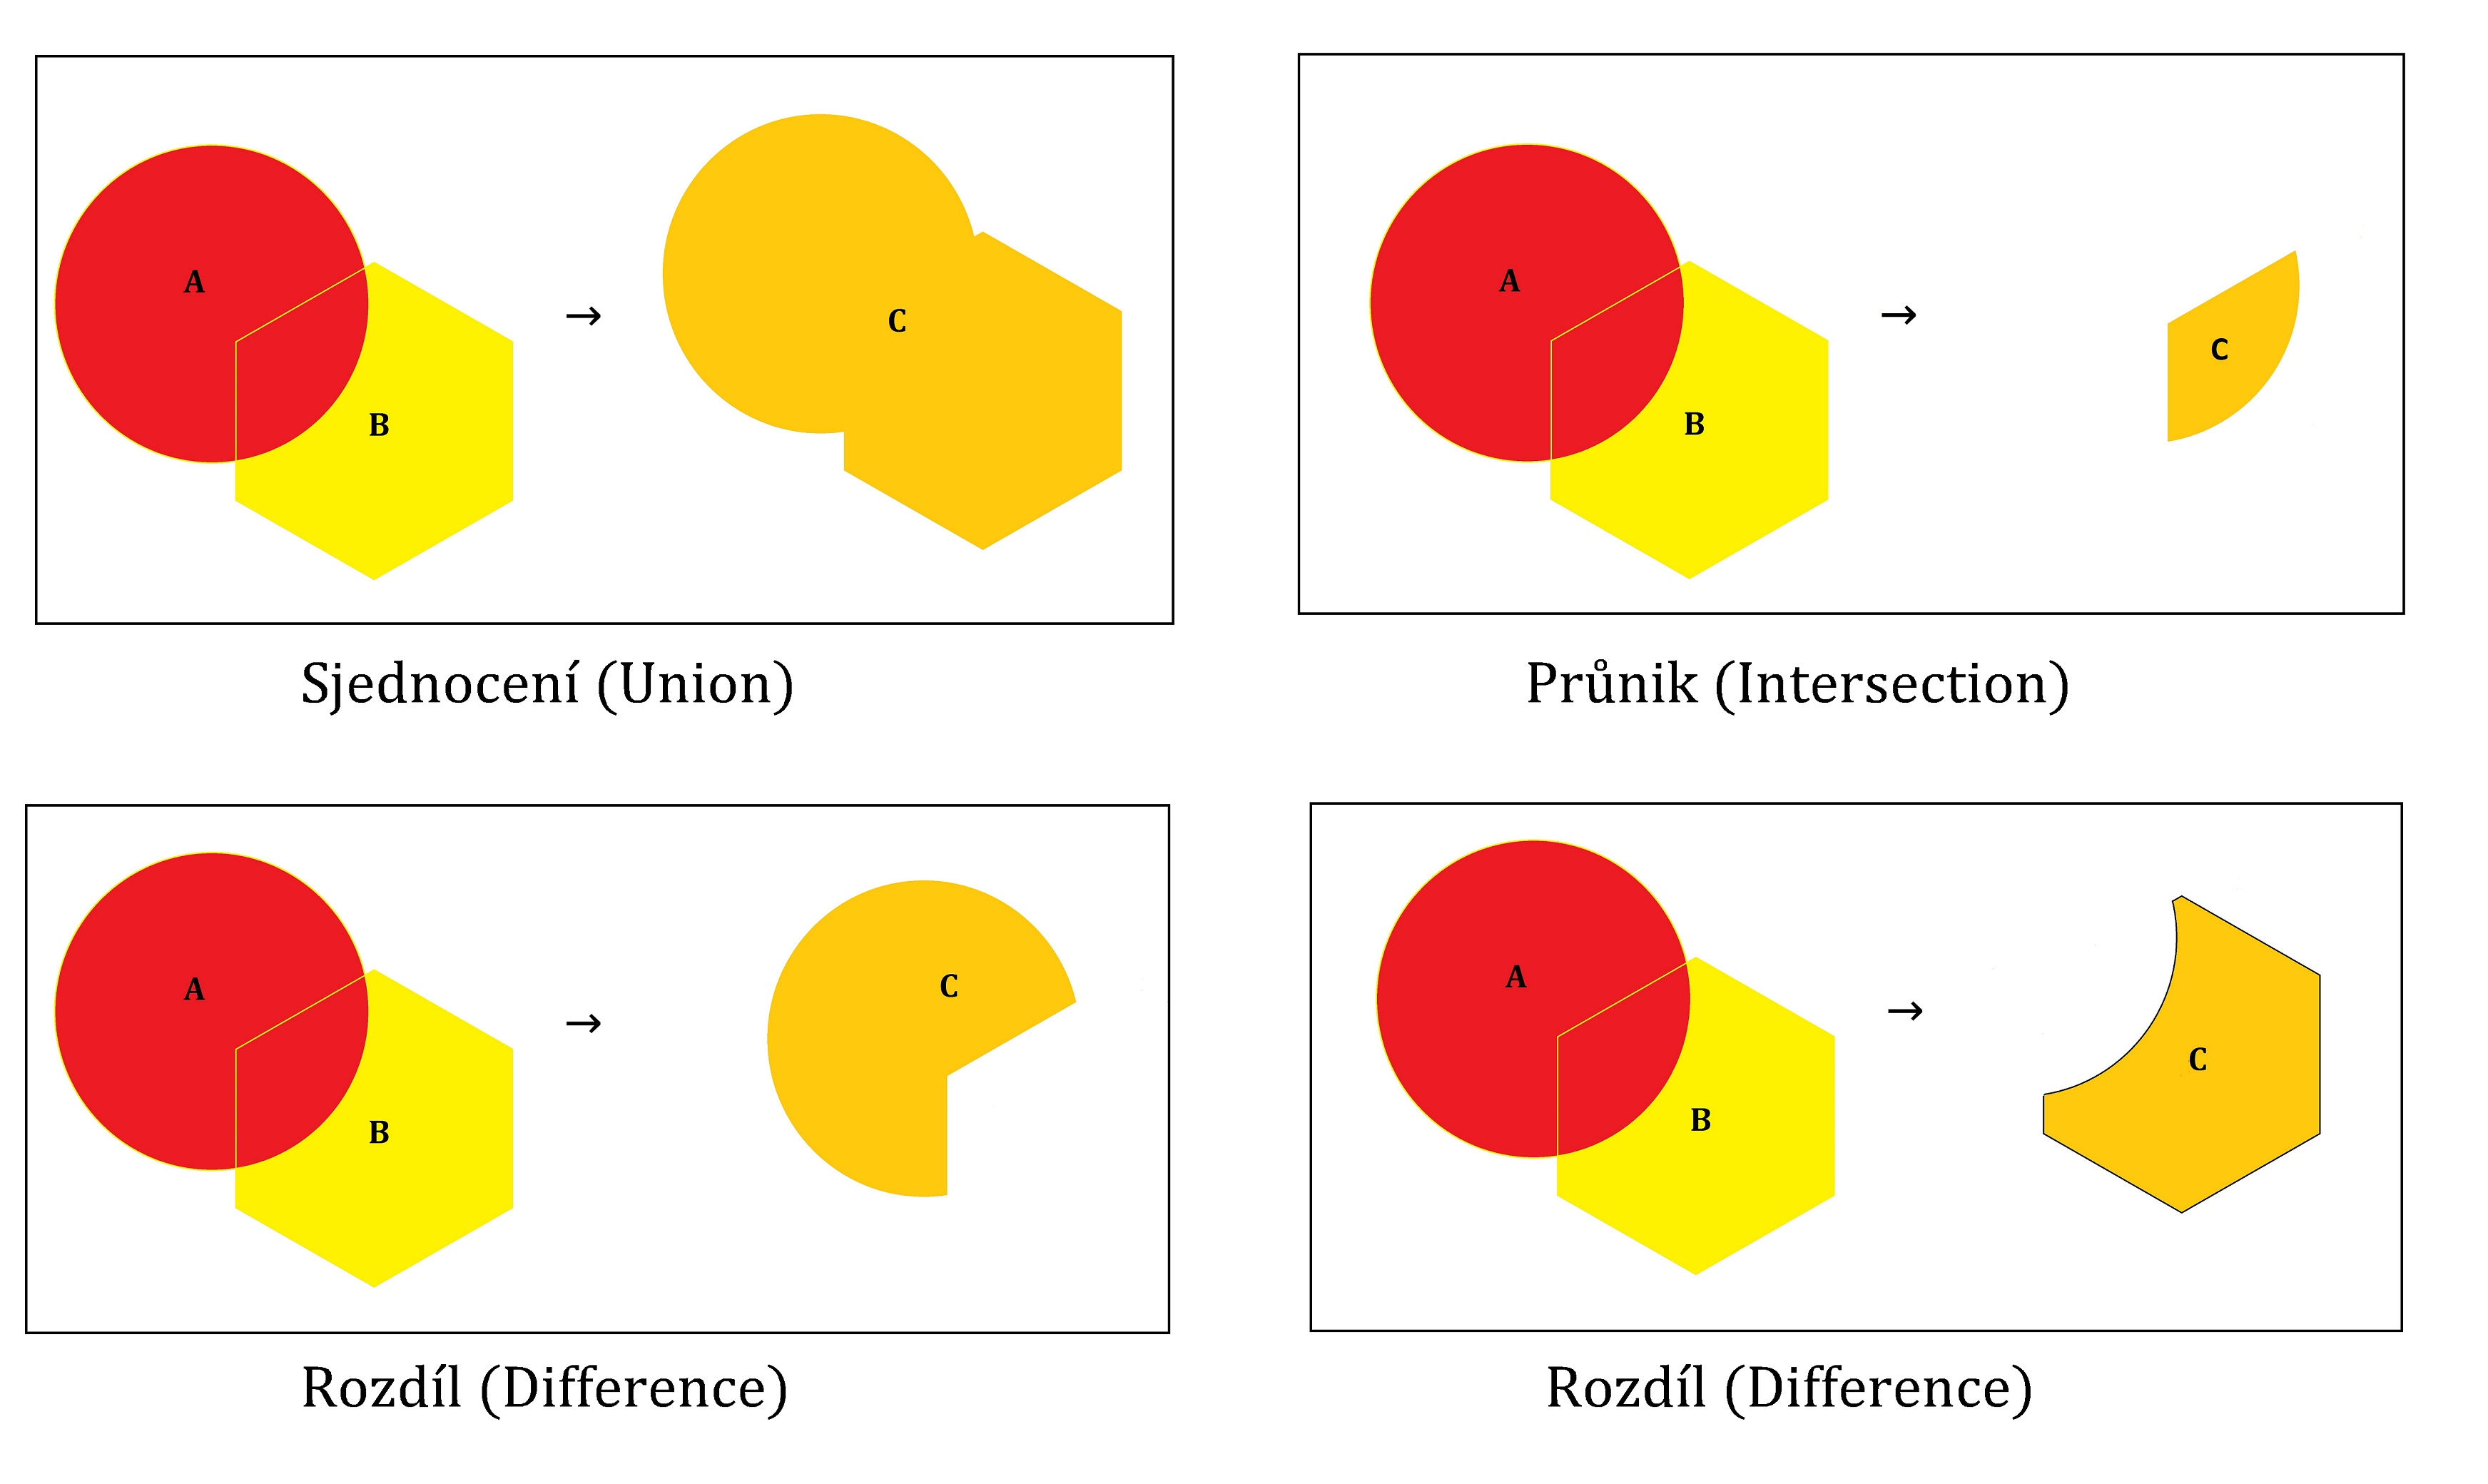
\includegraphics[width=18cm]{BO.jpg}
	\caption{Příklady množinových operací}
\end{figure}


\clearpage
\section{Popis algoritmů}

\subsection{Výpočet průsečíků}

\subsubsection{Implementace metody}
\begin{enumerate}
\item $ for (i = 0; i < n, i++) $ 
\item \hspace {1cm} $ M = map (double, QPointFB) $ // Vytvoření mapy 
\item \hspace {1cm} $ for (j = 0; j < m, j++) $
\item \hspace {2cm} if $ b_{ij} = (p_i, p_{(i+)1\%n} \cap q_j, q_{(j+)1\%m }) \neq 0$ // Existuje průsečík
\item \hspace {3cm} $ M [\alpha_i] \longleftarrow b_{ij}$ //Přidej do M
\item \hspace {3cm} ProcessIntersection $ (b_{ij}, \beta, B, j) $ //Zpracuj první průsečík pro $ e_j $
\item \hspace {1cm} if $(||M|| > 0)$ // Nějaké průsečíky jsme nalezli
\item \hspace{2cm} $  for \forall m \in M: $ // Procházej všechny průsečíky v M
\item  \hspace{3cm} $ b \longleftarrow m.second $ // Získej 2. hodnotu z páru
\item \hspace{3cm} ProcessIntersection $ (b, \alpha, A, i) $ //Zpracuj první průsečík pro $ e_i $
\end{enumerate}

\vspace{1cm}

\textbf{Process Intersection} 
\begin{enumerate}
	\item $ if (|t| < \epsilon): $ 
	\item \hspace {1cm} $ P[i] \longleftarrow inters $  //Startovní bod průsečíkem
	\item  $ if (|t-1| < \epsilon): $
	\item \hspace {1cm}  $ P[(i+1)\%m] \longleftarrow inters$ // Koncový bod průsečíkem
	\item  $ else:$
	\item \hspace {1cm} ProcessIntersection $ i \longleftarrow i+1 $ //Inkrementuj pozici
	\item \hspace {1cm} if $P \longleftarrow  (b,i)$ // Přidej průsečík na pozici i+1
\end{enumerate}

\clearpage

\subsection{Fragmenty}

\subsubsection{Vytvoření fragmentů - implementace metody}
\begin{enumerate}
	\item $ i \longleftarrow 0 $
	\item $ while (g(P[i]) \neq g \vee P[i] \neq inters) $ //Dokud P[i] není průsečík s orientací g
	\item \hspace{1cm} $ i \longleftarrow i+1 $
	\item $ if (i\equiv n) $ return; //Žádný bod s touto orientací neexistuje
	\item $ i_s \longleftarrow i $ //Zapamatuj startovní index prvního průsečíku
	\item $ do $
	\item \hspace{1cm} $ f = \emptyset $ //Prázdný fragment
	\item \hspace{1cm} $ if (createFragmentFromVertices (i_s, P, g, i f)) $ //Nalezen fragment
	\item \hspace{2cm} $ if (s) f.reverse() $ //Swapuj prvky fragmentu, je-li třeba
	\item \hspace{2cm} $ F[f[0]] \longrightarrow f $ //Přidej fragment do mapy, klíč poč. bod
	\item \hspace{1cm} $ i \longleftarrow (i+1)\%m $
	\item $ while (i \neq i_s) $ //Dokud nedojdeme k počátečnímu průsečíku
\end{enumerate}

\vspace{1cm}

\textbf{createFragmentFromVertices}

\begin{enumerate}
	\item  $ if (g(P[i]) \neq g \vee P[i] \neq inters) $ //Bod není průsečíkem s orientací g
	\item \hspace{1cm} $ return $ $ false $ 
	\item for (;;) 
	\item \hspace{1cm} $  f \longleftarrow P[i] $ // Přidej bod do fragmentu
	\item \hspace{1cm} $ i \longleftarrow (i+1)\%n $
	\item \hspace{1cm} $ if (i \equiv i_s) $ //Obešli jsme celý polygon
	\item \hspace{2cm} $ return$  $ false $ 
	\item \hspace{1cm} $ if (g(P[i]) \neq g)  $ // První bod s rozdílou orientací
	\item \hspace{2cm} $ f \longleftarrow P[i] $ //Přidej ho do seznamu
	\item \hspace{2cm} $ return$  $true $

\end{enumerate}

\clearpage

\subsubsection{Sestavení oblastí z fragmentů - implementace metody}
\begin{enumerate}
	\item $ for \forall f \in F $
	\item \hspace{1cm} $ P \longleftarrow \emptyset $ //Vytvoř prázdný polygon
	\item \hspace{1cm} $ s \longleftarrow f.first $ //Najdi startovní bod fragmentu
	\item \hspace{1cm} $ if (!f.second.first) $ //Pokud fragment již nebyl zpracován
		\item \hspace{2cm} $ if (createPolygonFROMFragments(s,F,P)) $ 
			\item \hspace{3cm} $ C \longleftarrow P $ //Přidej polygon do seznamu	
\end{enumerate}

\vspace{1.5cm}
\subsubsection{Vytvoření polygonu z fragmentů  - implementace metody}

\begin{enumerate}
	\item  $ QPoint n \longleftarrow s $ //Inicializuj následující bod
	\item for (;;) //Projdi všechyn fragmenty tvořící polygon
	\item \hspace{1cm} $ f \longleftarrow F.find(n) $ //Najdi navazující fragment
	\item \hspace{1cm} $ if (f \equiv F.end) $ // Fragment s takovým poč. bodem neexistuje
	\item \hspace{2cm} $ return$ $ false $
	\item \hspace{1cm} $ f.second.first \longleftarrow true $ //Fragment označen za zpracovaný
	\item \hspace{1cm} $ n \longleftarrow f.second.second.back() $ // Najdi následující bod
	\item \hspace{1cm} $ P \longleftarrow f.second.second - \{f.second.second[0]\}() $ // Přidej bez poč. bodu
	\item \hspace{1cm} $ if (n \equiv s) $ // Obešli jsme polygon, jsme na startu
	\item \hspace{2cm} $ return$  $true $
\end{enumerate}

\clearpage

\subsection{Množinové operace}

\subsubsection{Implementace metody}
\begin{enumerate}
	\item if $ (o(A) != CCW) $
	\item \hspace{1cm} $ A.switchOr() $ // Změň orientaci na CCW
	\item if $ (o(B) != CCW) $
	\item \hspace{1cm} $ B.switchOr() $ // Změň orientaci na CCW
	\item $ ComputeIntersections(A,B) $ // urči průsečíky A,B
	\item $ SetPositions (A,B) $ //Urči polohu vrcholů vůči oblastem
	\item $map <QPointFB, pair <bool, vector<QPointFB>>> F$
	\item $ pos1 = (oper \equiv intersection \vee oper \equiv DifAB?Inner:Outer) $
	\item $ pos2 = (oper \equiv intersection \vee oper \equiv DifAB?Inner:Outer) $
	\item $ swap1 = (oper \equiv DifAB? : true : false) $
	\item $ swap2 = (oper \equiv DifAB? : true : false) $
	\item $ CreateFragments (A, pos1, swap1, F) $
	\item $ CreateFragments (B, pos2, swap2, F) $
	\item $ MergeFragments (A,B,C) $
\end{enumerate}

\clearpage
% ===============================================================

\section{Vstupní data}


%--------------------------------------------------------------------------------------------------------------------------------------

\clearpage
\section{Ukázka vytvořené aplikace}

\clearpage

%=======================================================================================



\subsection{Algorithms}
V třídě Algorithms jsou staticky implementovány algoritmy počítající kovexní obálku a minimální ohraničující obdélník (včetně vodící linie).

\begin{itemize}

	\item Výčtový typ \textbf{TPosition}
		\begin{itemize}
			\item Typ využitý jako návratová hodnota členské metody \textbf{getPointLinePosition}.
			\item \textbf{LEFT = 0}
			\item \textbf{RIGHT = 1}
			\item \textbf{ON = 2}
		\end{itemize}

	\item Metoda \textbf{getPointLinePosition}
		\begin{itemize}
			\item Tato metoda slouží k určení polohy bodu vůči přímce. Návratovou hodnotou je výčtový typ \textbf{TPosition}.
			\item Vstup
				\begin{itemize}
					\item \textbf{QPointF \&q} - určovaný bod
					\item \textbf{QPointF \&a, \&b} - body přímky
				\end{itemize}
			\item Výstup
				\begin{itemize}
					\item \textbf{LEFT} - bod vlevo od přímky
					\item \textbf{RIGHT} - bod vpravo od přímky
					\item \textbf{ON} - bod na přímce
				\end{itemize}

		\end{itemize}

	\item Metoda \textbf{getTwoVectorsAngle}
		\begin{itemize}
			\item Tato metoda slouží k určení úhlu mezi 2 přímkami. Její návratovou hodnotu je \textbf{double}.
			\item Vstup
				\begin{itemize}
					\item \textbf{QPointF \&p1, \&p2} - body první přímky
					\item \textbf{QPointF \&p3, \&p4} - body druhé přímky
				\end{itemize}
		
			\item Výstup
				\begin{itemize}
					\item Úhel mezi 2 přímkami
				\end{itemize}			
		\end{itemize}

	\item Metoda \textbf{getPointLineDistance}
		\begin{itemize}
			\item Tato metoda slouží k výpočtu vzdálenosti bodu od přímky. Její návratovou hodnotou je \textbf {double} %\begin{double.}
			\item Vstup
				\begin{itemize}
					\item \textbf{QPointF \&q} - určovaný bod
					\item \textbf{QPointF \&a, \&b} - body přímky
				\end{itemize}
			\item Výstup
				\begin{itemize}
					\item Vzdálenost bodu od přímky
				\end{itemize}
		\end{itemize}

	\item Přetížená metoda \textbf{rotateByAngle}
		\begin{itemize}
			\item Tato metoda slouží k rotaci dané množiny o úhel. Jejím návratovým typem je \textbf{void}.
			\item Vstup
				\begin{itemize}
					\item Přetížení 1
						\begin{itemize}
							\item \textbf{std::vector$<$QPointF$>$ \&points} - vektor bodů, jež má být orotován
							\item \textbf{double angle} - úhel, o který má rotace být provedena
 						\end{itemize}
					
					\item Přetížení 2
						\begin{itemize}
							\item \textbf{QPolygonF \&points} - polygon, jež má být orotován
							\item \textbf{double angle} - úhel, o který má rotace být provedena
 						\end{itemize}

					\item Přetížení 3
						\begin{itemize}
							\item \textbf{QLineF \&points} - úsečka, jež má být orotována
							\item \textbf{double angle} - úhel, o který má rotace být provedena
 						\end{itemize}					
				\end{itemize}
			
		\end{itemize}

	\item Metoda \textbf{getDistance}
		\begin{itemize}
			\item Tato metoda slouží k výpočtu vzdálenosti dvou bodů. Jejím výstupním typem je \textbf{double}.
			\item Vstup
				\begin{itemize}
					\item \textbf{QPointF \&a, \&b} - body, mezi kterými je vzdálenost počítána
				\end{itemize}
			\item Výstup
				\begin{itemize}	
					\item Vypočtená vzdálenost
				\end{itemize}
		\end{itemize}

	\item Metoda \textbf{jarvisScanCH}
		\begin{itemize}
			\item Tato metoda slouží k výpočtu konvexní obálky pomocí algoritmu Jarvis Scan. Během výpočtu je ošetřována singularita existence kolineárních bodů v datasetu. Jejím výstupním typem je \textbf{QPolygonF}.
			\item Vstup
				\begin{itemize}
					\item \textbf{std::vector} $<$\textbf{QPointF}$>$ \textbf{points} - vektor bodů, kolem nichž má být vytvořená konvexní obálka.
				\end{itemize}
			\item Výstup
				\begin{itemize}
					\item Polygon obsahující kovexní obálku.
				\end{itemize} 
		\end{itemize}

	\item Metoda \textbf{grahamScanCH}
		\begin{itemize}
			\item Tato metoda slouží k výpočtu konvexní obálky pomocí algoritmu Graham Scan. Jejím výstupním typem je \textbf{QPolygonF}.
			\item Vstup
				\begin{itemize}
					\item \textbf{std::vector} $<$\textbf{QPointF}$>$ \textbf{points} - vektor bodů, kolem nichž má být vytvořená konvexní obálka.
				\end{itemize}
			\item Výstup
				\begin{itemize}
					\item Polygon obsahující kovexní obálku.
				\end{itemize} 
		\end{itemize}

	\item Metoda \textbf{quickHullCH}
		\begin{itemize}
			\item Tato metoda slouží k výpočtu konvexní obálky pomocí algoritmu Quick Hull. Jejím výstupním typem je \textbf{QPolygonF}.
			\item Vstup
				\begin{itemize}
					\item \textbf{std::vector} $<$\textbf{QPointF}$>$ \textbf{points} - vektor bodů, kolem nichž má být vytvořená konvexní obálka.
				\end{itemize}
			\item Výstup
				\begin{itemize}
					\item Polygon obsahující kovexní obálku.
				\end{itemize} 
		\end{itemize}

	\item Metoda \textbf{quickHullLocal}
		\begin{itemize}
			\item Pomocná metoda k výpočtu konvexní obálky metodou Quick Hull. Jejím výstupním typem je \textbf{void}.
			\item Vstup
				\begin{itemize}
					\item \textbf{int s, e} - index počátečního a koncového bodu dělící přímky
					\item \textbf{std::vector} $<$\textbf{QPointF}$>$ \&\textbf{points} - vektor bodů, kolem nichž má být vytvořená konvexní obálka.
					\item \textbf{QPolygonF \&poly\_ch} - polygon obsahující body konvexní obálky
				\end{itemize}
			\item Výstup
				\begin{itemize}
					\item Polygon obsahující kovexní obálku.
				\end{itemize} 
		\end{itemize}

	\item Metoda \textbf{sweepLineCH}
		\begin{itemize}
			\item Tato metoda slouží k výpočtu konvexní obálky pomocí algoritmu Sweep Line. Jejím výstupním typem je \textbf{QPolygonF}.
			\item Vstup
				\begin{itemize}
					\item \textbf{std::vector} $<$\textbf{QPointF}$>$ \textbf{points} - vektor bodů, kolem nichž má být vytvořená konvexní obálka.
				\end{itemize}
			\item Výstup
				\begin{itemize}
					\item Polygon obsahující kovexní obálku.
				\end{itemize} 
		\end{itemize}

	\item Metoda \textbf{generatePoints}
		\begin{itemize}
			\item Metoda pro generování zadaného počtu a tvaru bodů. Jejím výstupním typem je \textbf{std::vector} $<$\textbf{QPointF}$>$ \textbf{points}.
			\item Vstup
				\begin{itemize}
					\item \textbf{QSizeF \&canvas\_size} - rozměry kreslícího plátna, ze kterých se determinuje rozsah generovaných bodů
					\item \textbf{int point\_count} - počet bodů, který se má generovat
					\item \textbf{std::string shape} - tvar vytvářené množiny bodů (random, grid, na kružnici, na elipse, na čtverci)
				\end{itemize}
			\item Výstup
				\begin{itemize}
					\item Vektor nagenerovaných bodů.
				\end{itemize}
		\end{itemize}

	\item Metoda \textbf{minimalRectangle}
		\begin{itemize}
			\item Metoda pro výpočet minimálního ohraničujícího obdélníku a hlavní linie. Jejím výstupním typem je \textbf{void}.
			\item Vstup
				\begin{itemize}
					\item \textbf{QPolygonF \&poly\_ch} - polygon obsahující konvexní obálku
					\item \textbf{QPolygonF \&minimal\_rectangle} - polygon, do kterého jsou počítány body minimálního ohraničujícího obdélníku
					\item \textbf{QLineF \&direction} - hlavní linie minimálního ohraničujícího obdelníku (resp. do této proměnné je počítaná)
					\item \textbf{bool compute\_dir\_line} - ukazatel určující zda-li má být počítána hlavní linie minimálního ohraničujícího obdélníku
				\end{itemize}

		\end{itemize}
\end{itemize}
\clearpage

\subsection{Draw}
Třída draw slouží k vykreslení vygenerovaných (nebo naklikaných) bodů, vypočteného minimálního ohraničujícího obdélníku a hlavní linie minimálního ohraničujícího obdélníku. V této třídě jsou zároveň nagenerované body zbavené duplicit a vypočtené konvexní obálky se zde omezují na striktní konvexní obálky (vše v metodě \textbf{setCH}. Třída dědí od třídy \textbf{QWidget}. 

\begin{itemize}
	\item Členské proměnné
		\begin{itemize}
			\item \textbf{std::vector} $<$\textbf{QPointF}$>$ \textbf{points} - vektor obsahující nagenerované nebo naklikané body
			\item \textbf{QPOlygonF ch} - polygon obsahující body konvexní obálky
			\item \textbf{QPolygonF rect} - polygon obsahující body minimálního ohraničujícího obdélníku
			\item \textbf{QLineF direction} - hlavní linie minimálního ohraničujícího obdélníka
		\end{itemize}

	\item Metoda \textbf{paintEvent}
		\begin{itemize}
			\item Tato metoda slouží k vykreslení nagenerovaných (nebo naklikaných) bodů, konvexní obýlky, minimálního ohraničujícího obdélníka a hlavní linie minimálního ohraničujícího obdélníka. Metoda se volá pomocí metody \textbf{repaint()}. Návratovým typem je \textbf{void}.
			\item Vstup
				\begin{itemize}
					\item \textbf{QPaintEvent *e}
				\end{itemize}
		\end{itemize}

	\item Metoda \textbf{mousePressEvent}
		\begin{itemize}
			\item Metoda sloužící k uložení bodu do členské proměnné \textbf{points} určeného kliknutím myší nad kreslícím plátnem. Jejím návratovým typem je \textbf{void}.	
			\item Vstup
				\begin{itemize}
					\item \textbf{QMouseEvent *e}
				\end{itemize}
		\end{itemize}

	\item Metoda \textbf{setCH}
		\begin{itemize}
			\item Tato metoda slouží pro kontrolu duplicity generovaných bodů, pro kontrolu alespoň 3 bodů, k zavolání příslušného algoritmu pro vypočtení konvexní obálky a k omezení konvexní obálky na striktně konvexní obálku. Metoda počítá dobu trvání výpočetních algoritmů. Jejím návratovým typem je \textbf{double}.
			\item Vstup
				\begin{itemize}
					\item \textbf{std::string \&selected\_algorithm} - uživatelsky vybraný algoritmus pro počítání konvexní obálky
				\end{itemize}
			\item Výstup
				\begin{itemize}
					\item Čas trvání výpočtu.
				\end{itemize}
		\end{itemize}	

	\item Metoda \textbf{setRect}
		\begin{itemize}
			\item Tato metoda slouží pro zavolání algoritmu pro výpočte minimálního ohraničujícího obdélníku a jeho hlavní linie. Jejím návratovým typem je \textbf{void}.
			\item Vstup
				\begin{itemize}
					\item \textbf{bool draw\_dir\_line} - uživatelsky nastavený indikátor, zda-li se má vypočítat hlavní linie minimálního ohraničujícího obdélníku
				\end{itemize}
		\end{itemize}

	\item Metoda \textbf{setPoints}
		\begin{itemize}
			\item Metoda volající algoritmus pro generování bodů daného počtu a tvaru. Jejím návratovým typem je \textbf{void}.
			\item Vstup
				\begin{itemize}
					\item \textbf{QSizeF \&canvas\_size} - rozměr kreslícího plátna pro pozdější určení rozsahu generování bodů
					\item \textbf{int count} - počet bodů, jež se má generovat
					\item \textbf{std::string \&shape} - tvar, do kterého se body mají generovat
				\end{itemize}
		\end{itemize}

	\item Metoda \textbf{clearCanvas}
		\begin{itemize}
			\item Metoda, která maže obsah kreslícího okna. Jejím návratovým typem je \textbf{void}. Do metody nevstupují žádné parametry.
		\end{itemize}
\end{itemize}

\subsection{SortByXAsc, SortByYAsc, SortByAngleAsc}
Třídy sloužící jako sortovací kritérium - podle rostoucí souřadnice x resp. souřadnice y (při stejných souřadnicích x resp. y je druhým kritériem druhá souřadnice) a podle rostoucího úhlu mezi body (při stejném úhlu je druhým kritériem vzdálenosti mezi body).
\clearpage

\subsection{Widget}
Tato třída slouží ke komunikaci s GUI. Třída dědí od třídy QWidget. Všechny její metody slouží jako sloty k signálům z GUI, nemají žádné vstupní hodnoty a jejich návratovým typem je void. 

\begin{itemize}
	\item Metoda \textbf{on\_createCHButton\_clicked} - reaguje na zmáčknutí tlačítka pro vypočtení konvexní obálky, volá metodu \textbf{setCH} z třídy \textbf{Draw}, zapisuje čas výpočtu do GUI.

	\item Metoda \textbf{on\_generateButton\_clicked} - reaguje na zmáčknutí tlačítka pro generování bodů, volá metodu \textbf{setPoints} z třídy \textbf{Draw}.

	\item Metoda \textbf{on\_clearButton\_clicked} - reaguje na zmáčknutí tlačítka pro vymazání obsahu kreslícího plátna, volá metodu \textbf{clearCanvas} z třídy \textbf{Draw}.

	\item Metoda \textbf{on\_createRectButton\_clicked} - reaguje na zmáčknutí tlačítka pro vypočtení minimálního ohraničujícího obdélníka, volá metodu \textbf{setRect} z třídy \textbf{Draw}.

	\item Metoda \textbf{on\_helpButton\_clicked} - reaguje na zmáčknutí tlačítka pro volání nápovědy, volá okno s nápovědou \textbf{help\_dialog} z třídy \textbf{HelpDialog}.

\end{itemize} 

\vspace{3cm}
\subsection{HelpDialog}
Třída sloužící pro vykreslení okna s nápovědou.

\clearpage

\section{Přílohy}

\begin{itemize}
	\item Príloha č.1: Testování výpočetních dob algoritmů - "Testovani.pdf"
\end{itemize}
 %--------------------------------------------------------------------------------------------------------------------------------------------------------------------------
\clearpage
\section{Závěr}

\subsection{Návrhy na vylepšení}

\begin{itemize}
\item bla bla
\end{itemize}

\clearpage
\section{Zdroje}

\begin{enumerate}
\item  BAYER, Tomáš. Konvexní obálky [online][cit. 3.1.2019]. \\
Dostupné z: https://web.natur.cuni.cz/~bayertom/images/courses/Adk/adk9.pdf  \\

\item  BAYER, Tomáš. Konvexní obálky [online][cit. 3.1.2019]. \\
Dostupné z: https://web.natur.cuni.cz/~bayertom/images/courses/Adk/adkcv4.pdf\\
%=======================================================================================
\end{enumerate}
\end{document}



 
